%! Author = itgramic
%! Date = 24.11.23

% Preamble
\chapter{Testsystem}
\begin{flushleft}
    Bevor der Patch eingespielt werden kann, müssen die Voraussetzungen erfüllt sein.
    Da das Testsystem im laufenden Betrieb gepatched wird und Standardmässig die \texttt{Workstation.exe} für das Testsystem nur auf dem Laufwerk \texttt{K:\textbackslash} steht, muss ein Lokales verzeichnis im \texttt{C:\textbackslash} erstellt werden.
\end{flushleft}
\begin{flushleft}
    Ausserdem sollten zwei Ini-Files präperiert werden.\\
    \textbf{sks0060}\\
    \lstset{style=gra_codestyle}
    \begin{lstlisting}[language=sh, caption=Workstation.ini TEST sks0060,captionpos=b,label={lst:workstation.ini-test-sks0060},breaklines=true]
    -clean
    -data
    @noDefault
    -configuration
    C:\temp\phoenix\test1_7_23_1\eclipse\configuration
    -nl
    de_CH
    -vmargs
    -Dorg.eclipse.update.reconcile=false
    -Dphoenix.db=Phoenix_Test1
    -Dphoenix.application.workspace.createdir=true
    -Dphoenix.application.workspace=\\\\phoenix\workspace\test1_7_23_1
    -Dphoenix.login.usernamefile=%APPDATA%/Phoenix/login_username_test1
    -Dphoenix.server.nodes=sks0060:8443
    -Djavax.net.ssl.trustStore=.\truststore.jks
    -Dphoenix.login.enableLDAP=true
    -Dphoenix.application.winlogin=true
    -Dphoenix.g3his.url=http://clinical-qa.ksgr.ch:8280/cgmg3
    \end{lstlisting}
    \textbf{sks0103}\\
    \lstset{style=gra_codestyle}
    \begin{lstlisting}[language=sh, caption=Workstation.ini TEST sks0103,captionpos=b,label={lst:workstation.ini-test-sks0103},breaklines=true]
    -clean
    -data
    @noDefault
    -configuration
    C:\temp\phoenix\test1_7_23_1\eclipse\configuration
    -nl
    de_CH
    -vmargs
    -Dorg.eclipse.update.reconcile=false
    -Dphoenix.db=Phoenix_Test1
    -Dphoenix.application.workspace.createdir=true
    -Dphoenix.application.workspace=\\\\phoenix\workspace\test1_7_23_1
    -Dphoenix.login.usernamefile=%APPDATA%/Phoenix/login_username_test1
    -Dphoenix.server.nodes=sks0103:8443
    -Djavax.net.ssl.trustStore=.\truststore.jks
    -Dphoenix.login.enableLDAP=true
    -Dphoenix.application.winlogin=true
    -Dphoenix.g3his.url=http://clinical-qa.ksgr.ch:8280/cgmg3
    \end{lstlisting}
    \begin{mdframed}
    Vorsichht!\\Bei jedem KIS Phoenix Test1 Update kann sich die Konfiguration ändern!\\Daher sollten die Inis immer neu generiert werden bei den Updates.
    \end{mdframed}
\end{flushleft}
\begin{flushleft}
    Folgende Schritte müssen gemacht werden, um den Patch durchzuführen:
    \begin{enumerate}
        \item Snapshost der beiden Server \texttt{sks0060} und \texttt{sks0103} machen
        \item Prüfen ob \texttt{Workstation.exe Test1} auf \texttt{sks0060} und \texttt{sks0103} verbinden kann
        \item Prüfen ob \texttt{Workstation.exe Test1} nur auf \texttt{sks0103} verbinden kann
        \item Den Dienst \texttt{PhoenixJBossEAP\_test1\_1} auf \texttt{sks0060} stoppen
        \item Server \texttt{sks0060} rebooten
        \item Auf \texttt{sks0060} prüfen, ob keine Patches mehr gezogen werden könnten
        \item Prüfen ob \texttt{Workstation.exe Test1} auf \texttt{sks0060} verbinden kann
        \item Prüfen ob \texttt{Workstation.exe Test1} auf \texttt{sks0103} verbinden kann
        \item Prüfen ob \texttt{Workstation.exe Test1} auf \texttt{sks0060} und \texttt{sks0103} verbinden kann
        \item Den Dienst \texttt{PhoenixJBossEAP\_test1\_2} auf \texttt{sks0103} stoppen
        \item Server \texttt{sks0103} rebooten
        \item Auf \texttt{sks0103} prüfen, ob keine Patches mehr gezogen werden könnten
        \item Prüfen ob \texttt{Workstation.exe Test1} auf \texttt{sks0103} verbinden kann
        \item Prüfen ob \texttt{Workstation.exe Test1} auf \texttt{sks0060} verbinden kann
        \item Prüfen ob \texttt{Workstation.exe Test1} auf \texttt{sks0060} und \texttt{sks0103} verbinden kann
        \item Wenn die Tests erfolgreich waren, Snapshost der beiden Server \texttt{sks0060} und \texttt{sks0103} löschen
    \end{enumerate}
\end{flushleft}
\begin{flushleft}
    Das ganze noch als Sequenzdiagramm dargestellt:
    \begin{figure}[H]
        \centering
        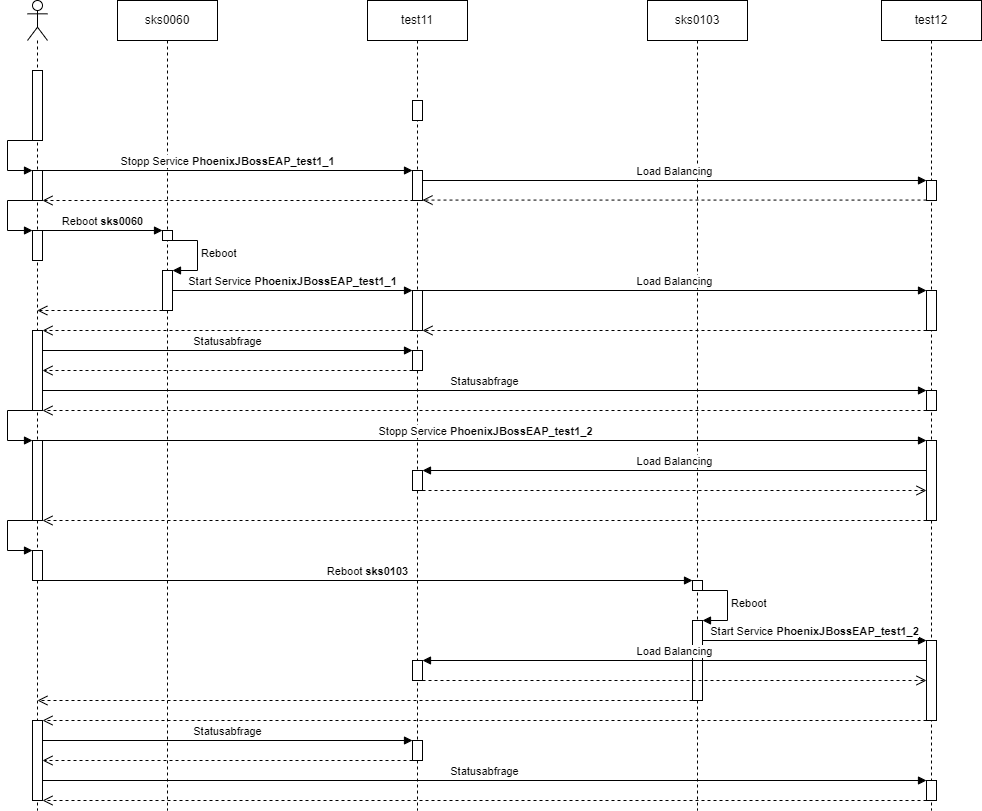
\includegraphics[width=1\linewidth]{source/test/sequenzdiagramm_test}
        \caption{TEST-Sequenzdiagramm}
        \label{fig:test-sequenzdiagramm}
    \end{figure}
\end{flushleft}
\begin{flushleft}

\end{flushleft}
